% Font size, paper type
\documentclass[12pt]{article}
% Aesthetic margins
\usepackage[margin=1in]{geometry}
% Core math packages,
% Mathtools loads amsmath, and amsmath gives basic math symbs
% Amsfonts & amssymb are misc. symbols you might need
\usepackage{mathtools, amsfonts, amssymb}
% Links in a pdf
\usepackage{hyperref}
% Use in pictures, graphs, and figures
\usepackage{graphicx}
% Header package
\usepackage{fancyhdr}
% Underlining with line breaks
\usepackage{ulem}
% Adjust accordingly given warning messages
\setlength{\headheight}{15pt}
% So we can more easily format text with pictures
\usepackage{float}

% Sets footer
\pagestyle{fancy}
% Removes default footer style
\fancyhf{}

\rhead{
  Shengdong Li
  Calc 3
}

\rfoot{
  Page \thepage
}

% Makes links look more appealling
\hypersetup{
    colorlinks=true,
    linkcolor=blue,
    filecolor=magenta,      
    urlcolor=cyan,
}

% \usepackage{indentfirst}

\begin{document}
\title{In Conclusion}
\author{by Shengdong Li}
\date{20 December 2020}
\maketitle


In this discussion, I had multiple moments of surprise, from learning that the epicycloid could transform into at least two of the curves in the discussion.

First was from Westin's comment, when I learned that the asteroid graph, which could appear when the ratio of $a$ to $b$ was $4$, and $a$ was negative. This also made me realize that the ratio of $\left|\frac{a}{b}\right|$ actually determines the vertices of the epicycloid.

Next was from Deyvik's comment about the cardioid, which you could get by substituting the same $a$ and $b$, into the epicycloid equation.

My second derivative was really complicated and I'm not even sure if I simplified it all the way, but the concavity changes constantly in the epicycloid.

Finally, here's some art of an epicycloid

\begin{figure}[H]
  \begin{center}
    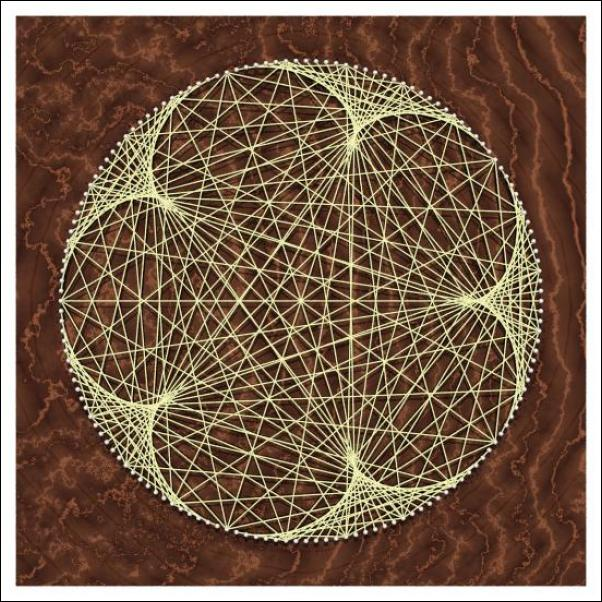
\includegraphics[scale=.3]{1.jpg}
  \end{center}
\end{figure}

\end{document}